\documentclass[conference]{IEEEtran}
\IEEEoverridecommandlockouts

% Essential IEEE Conference Packages
\usepackage{cite}
\usepackage{amsmath,amssymb,amsfonts}
\usepackage{algorithmic}
\usepackage{graphicx}
\usepackage{textcomp}
\usepackage{xcolor}
\usepackage{booktabs}
\usepackage{url}
\usepackage{microtype}
\usepackage[hidelinks]{hyperref}

\def\BibTeX{{\rm B\kern-.05em{\sc i\kern-.025em b}\kern-.08em
    T\kern-.1667em\lower.7ex\hbox{E}\kern-.125emX}}

\begin{document}

\title{RestockIQ: Empirical Demand Forecasting and Stochastic Inventory Simulation for Perishable Artisan Retail}

\author{
\IEEEauthorblockN{Yatin Patil}
\IEEEauthorblockA{\textit{Department of Information Technology} \\
\textit{SVKM's NMIMS Shirpur Campus}\\
Shirpur, Maharashtra, India \\
yatinpatilyp07@gmail.com}
\and
\IEEEauthorblockN{Soumy Raghuvanshi}
\IEEEauthorblockA{\textit{Department of Information Technology} \\
\textit{SVKM's NMIMS Shirpur Campus}\\
Shirpur, Maharashtra, India \\
soumyraghuvanshi@gmail.com}
\and
\IEEEauthorblockN{Chinmay Patil}
\IEEEauthorblockA{\textit{Department of Information Technology} \\
\textit{SVKM's NMIMS Shirpur Campus}\\
Shirpur, Maharashtra, India \\
chinmaygpatil04@gmail.com}
\and
\IEEEauthorblockN{Dr. Srikanth Pulipeti}
\IEEEauthorblockA{\textit{Head of Department, Dept. of Information Technology} \\
\textit{SVKM's NMIMS Shirpur Campus}\\
Shirpur, Maharashtra, India \\
srikanth.p@nmims.edu}
}

\maketitle

\begin{abstract}
Small-to-medium retail enterprises (SMEs) face acute challenges in managing perishable inventory under asymmetric demand costs. Over-ordering generates physical waste, while under-ordering causes lost sales margin and customer churn. In this study, we present an empirical evaluation of RestockIQ, an inventory intelligence system benchmarked on 637 calendar days (600 trading days) of transaction data from a commercial artisan bakery in France. The operational production deployment relies on a lightweight 30-day statistical baseline engine. In offline benchmarks across 38 weekly rolling-origin temporal folds, an autoregressive day-ahead gradient boosted decision tree (day-ahead GBDT, implemented via \texttt{HistGradientBoostingRegressor}) achieves 25.48\% pooled WAPE, outperforming the baseline Prophet model (27.95\% WAPE) across 27 of 38 folds (+2.47 percentage point error reduction, 95\% cluster CI [+0.49, +4.76]). Exogenous numerical weather forecast regressors deliver no statistically reliable predictive improvement across all 38 folds (pooled WAPE 27.63\%, 95\% cluster CI [$-$0.24, +0.87], $p = 0.3800$), and circular permutation placebo tests provide no evidence of usable signal beyond seasonal calendar indicators. In trace-driven stochastic Newsvendor inventory simulations across 88 operating days (68,883 demand units), a critical-ratio policy ($\text{CR}=0.60$ under 40\% cost-of-goods-sold) applied to the day-ahead GBDT achieves EUR~41,635.90 in gross profit with a 12.65\% waste rate and an 89.99\% unit fill rate. When evaluated against a conventional 95\% target service-level policy, the critical-ratio policy reduces food waste by 16,243 units ($-$64.4\%) and increases profit by EUR~5,839.55 (+16.3\%), while fill rate declines by 6.57 percentage points. Conversely, evaluated against an unbuffered zero-buffer policy ($z=0.0$), the critical-ratio policy raises profit by EUR~168.93 and improves fill rate from 87.58\% to 89.99\% at the cost of 2,084 additional waste units (with 7-day moving average baselines exhibiting lower profit under critical-ratio buffering). We discuss architectural trade-offs, operational limitations, and the practical deployment gap separating offline prototypes from live retail point-of-sale systems.
\end{abstract}

\begin{IEEEkeywords}
Perishable inventory, demand forecasting, Newsvendor model, gradient boosted trees, food waste reduction, retail operations.
\end{IEEEkeywords}

\section{Introduction}
\label{sec:intro}
Perishable retail goods have single-day operational shelf lives and volatile demand patterns. Small bakery and food service retailers must place daily production and replenishment orders prior to morning store opening \cite{gartner2024automated}. Unsold baked units at store closing cannot be inventoried for subsequent trading days and must be discarded as physical waste \cite{chowdhury2025predictive}. In contrast, morning and afternoon stockouts result in permanent sales losses and diminished customer retention \cite{access2025supply}.

Frontline store managers frequently rely on informal heuristics, such as static moving averages or subjective intuition \cite{cherian2025demand}. Although recent literature explores advanced machine learning architectures for retail demand prediction \cite{ganguly2024enhancing, jatte2025optimization}, a persistent operational gap remains between point forecast accuracy metrics and downstream restocking decisions \cite{groene2024introduction}. Replenishment policies require calibrated uncertainty estimates to balance underage costs (unrealized gross margin) against overage costs (spoilage and disposal) under asymmetric margins \cite{avuduri2025smartstock}.

Furthermore, retail studies frequently incorporate external meteorological regressors without counterfactual or placebo validation \cite{lalitha2025enhanced, jain2024weather}. Predictive models require rigorous falsification to establish whether exogenous weather features provide usable signal beyond seasonal calendar trends.

In this paper, we study the RestockIQ platform through an offline empirical evaluation on 637 calendar days of transaction data from an artisan bakery in Western France. Our investigation addresses four primary contributions:
\begin{enumerate}
    \item We execute an empirical multi-horizon demand forecasting benchmark across 38 weekly rolling-origin temporal folds, demonstrating that day-ahead autoregressive gradient boosted trees achieve 25.48\% pooled WAPE (+2.47 percentage points over a baseline Prophet generalized additive model).
    \item We conduct a circular permutation placebo test evaluating numerical weather forecast regressors, demonstrating that weather features offer no statistically reliable predictive gain (+0.32 pp, 95\% cluster CI [$-$0.24, +0.87], $p = 0.3800$).
    \item We conduct trace-driven single-period Newsvendor inventory simulations over 88 trading days under explicit operational assumptions (40\% COGS, single-day shelf life, zero salvage, and in-sample residual variance), benchmarking both against a 95\% service-level policy and an unbuffered zero-safety-stock baseline.
    \item We document the practical deployment gap between offline day-ahead research prototypes and the lightweight statistical baseline engine currently operating in production.
\end{enumerate}

\section{Related Work}
\label{sec:related}
We contextualize our study within four major streams of recent retail operations literature: time series forecasting benchmarks, perishable inventory control, exogenous environmental regressors, and operational AI adoption within small-to-medium enterprises.

\subsection{Retail Demand Forecasting Benchmarks}
Time series forecasting in retail environments spans classical statistical heuristics and supervised machine learning regressors \cite{access2025supply, gartner2024automated}. Classical moving averages and seasonal naive formulations provide robust, computation-free baselines for small retailers \cite{susanto2023performance}. Comparative studies on food service transaction series indicate that while statistical formulations such as SARIMA and additive decomposition models like Facebook Prophet \cite{taylor2018forecasting} capture weekly periodicity effectively, recurrent neural architectures (e.g., LSTM) capture non-linear intra-day dynamics \cite{iccraids2026comparative, munawar2026lstm}. Empirical evaluations demonstrate that gradient-boosted decision trees (GBDTs) \cite{friedman2001greedy}, including implementations via scikit-learn \cite{pedregosa2011scikit}, frequently achieve superior predictive accuracy on tabular retail sales data while maintaining low training latency \cite{ganguly2024enhancing, sandeep2023smart, jatte2025optimization}. Furthermore, recent investigations examine hybrid architectures combining additive seasonal decomposition with residual boosted learning to address multi-scale seasonality and SKU cross-correlations \cite{iciptm2026predictive, ictmod2025state, iccraids2026evaluation}.

\subsection{Perishable Inventory Control and Waste Reduction}
Perishable goods management requires balancing on-shelf product availability against physical discard \cite{chowdhury2025predictive, iconstem2025aidriven}. In food retail and restaurant settings, applying arbitrary fixed service-level targets (such as a 95\% in-stock target) forces excessive safety buffers, resulting in severe physical inventory discard and eroded profit margins \cite{avuduri2025smartstock}. Classical stochastic inventory control, formalized by the single-period Newsvendor framework \cite{arrow1951optimal}, balances underage costs against overage costs \cite{cherian2025demand}. Modern extensions connect point forecasts and residual uncertainty distributions directly into cost-optimal order fractiles, yet empirical evaluations rarely bridge offline forecasting models with full trace-driven replenishment simulations \cite{chowdhury2025predictive}.

\subsection{Exogenous Covariates and Weather Effects}
A substantial body of literature investigates the impact of local meteorological factors on consumer foot traffic and purchasing patterns \cite{guler2023forecasting, lalitha2025enhanced}. Variations in temperature, rainfall, and solar irradiance have been proposed as explanatory features for food and beverage demand fluctuations \cite{jain2024weather}. Nonetheless, meteorological features often exhibit high collinearity with seasonal calendar indicators and day-of-week trends \cite{guler2023forecasting}. Without counterfactual and placebo falsification tests, predictive gains attributed to weather regressors may reflect seasonal overfitting rather than genuine atmospheric causal effects \cite{lalitha2025enhanced}.

\subsection{Operational AI Adoption in SMEs}
Deploying predictive systems into small retail businesses presents practical challenges that differ markedly from enterprise-scale supply chains \cite{groene2024introduction}. Store managers frequently lack specialized technical training and distrust opaque automated decision mechanisms \cite{yuniarty2025technology}. Consequently, recent studies emphasize lightweight mobile point-of-sale interfaces and intuitive replenishment dashboards to lower the barrier to operational adoption \cite{icci2026mobile, icalter2024mobile}. Concurrently, foundation models and automated analytics are emerging as tools to support supply chain decision-making in small enterprises \cite{sera2025optimizing}. Moreover, food supply chain transparency and traceability have emerged as critical drivers of managerial trust and operational compliance in micro, small, and medium enterprises (MSMEs) \cite{timesicon2025technology}.

\section{Data Audit}
\label{sec:data}
The empirical dataset utilized in this investigation consists of anonymized daily point-of-sale transaction logs from a commercial artisan bakery in Western France. The observation window spans 637 continuous calendar days between January 2, 2021, and September 30, 2022.

\subsection{Operating Calendar and Trading Days}
Across the 637 calendar days, the store recorded active transactions on exactly 600 trading days. The remaining 37 calendar days recorded zero transactions and are treated as store closures. Forensically, 29 of the 37 zero-sale days occurred on Wednesdays (representing 29 zero-sale occurrences across the 91 Wednesdays in the observation period), while the remaining 8 zero-sale days occurred across other weekdays. Rather than assuming a rigid six-day operating week or attributing non-trading days to holiday schedules, all 37 zero-sale days are treated as closures and excluded from training and evaluation datasets, rather than being imputed as zero-demand observations.

\subsection{Catalog and SKU Stratification}
The recorded retail catalog comprises 148 distinct product references. Retail sales volume is heavily concentrated among core staple items. The top 35 primary SKUs account for 91.6\% of total unit sales volume and 79.3\% of total recorded revenue. The remaining 113 intermittent items represent slow-moving pastries, specialized confectionery, or catering orders with zero sales on most operating days. Our primary forecasting benchmark and inventory simulations focus on these 35 high-volume primary SKUs, selected based on cumulative sales volume across the recording window (which we explicitly analyze as a catalog look-ahead limitation in Section~\ref{sec:discuss}).

\subsection{Dataset Provenance and Meteorological Covariates}
The transaction records comprise an anonymized historical point-of-sale dataset from an artisan retail bakery in Western France, capturing daily customer basket receipts across the observation period. Meteorological covariates are sourced from the Open-Meteo Historical Forecast API for Guérande, France ($47.3275^\circ\text{ N}, -2.4289^\circ\text{ W}$), blending numerical weather prediction models (DWD ICON and ECMWF).

\section{System Architecture and Methodology}
\label{sec:method}

\subsection{Production System Overview}
RestockIQ is architected as an end-to-end inventory management platform for retail store managers. The production deployment comprises four decoupled tiers:
\begin{enumerate}
    \item \textbf{Mobile Client:} A Flutter application providing inventory monitoring and manual order adjustment screens.
    \item \textbf{Backend Microservice:} A FastAPI service hosted on Render managing inventory catalog state, user authentication, and forecast retrieval.
    \item \textbf{Database Tier:} A MongoDB Atlas cloud cluster (M0 free tier) storing item catalogs and pre-computed forecast documents.
    \item \textbf{Batch Execution Engine:} An automated nightly GitHub Actions cron workflow executing at 02:00 UTC. The production batch engine runs a 30-day trailing statistical baseline with day-of-week ratio multipliers and static safety buffers ($z=1.65$). The daily batch script also calls Google Gemini to generate natural language daily briefing summaries.
\end{enumerate}
\textbf{Crucially, the deployed production engine is strictly this 30-day statistical baseline. The day-ahead gradient boosted tree models evaluated in this paper represent offline research prototypes and are not deployed to live production.}

\subsection{The Deployment Gap}
A significant operational gap separates the offline research models from the operational production pipeline. Specifically, the live point-of-sale infrastructure does not yet implement an automated end-of-day sales rollup service. In live operations, customer sales are logged as individual basket line items. The offline day-ahead GBDT requires realized demand $y(t-1)$ to be aggregated, validated, and ingested before 02:00 UTC each morning. Because this automated pipeline does not exist in the production environment, the day-ahead GBDT cannot currently execute in production without manual data curation.

\subsection{Model Specifications and Hyperparameters}
Table~\ref{tab:model_defs} details the mathematical architecture, feature inputs, demand lags, training windows, and fixed hyperparameters across all evaluated models. All gradient-boosted decision trees are implemented using scikit-learn's \texttt{HistGradient\-Boosting\-Regressor} with fixed hyperparameters: learning rate $\eta = 0.05$, maximum iterations $M = 200$, maximum tree depth $d = 6$, random seed 42, and least-squares loss, with the article identifier declared as a categorical feature.

\begin{table*}[!t]
\centering
\caption{Systematic Model Specification and Hyperparameter Summary}
\label{tab:model_defs}
\resizebox{\textwidth}{!}{%
\begin{tabular}{lp{4.6cm}p{3.2cm}lp{3.6cm}c}
\toprule
\textbf{Model Key} & \textbf{Feature Inputs} & \textbf{Autoregressive Lags} & \textbf{Training Window} & \textbf{Hyperparameters / Estimation} & \textbf{Forecast Horizon} \\
\midrule
\texttt{prophet\_only} & Trend, weekly/yearly Fourier seasonality, French public holidays, tourist season multiplier & None & Expanding ($t \le \text{cutoff}$) & Multiplicative seasonality, default Prophet priors & 7-day origin \\
\texttt{model\_b\_cal} & Prophet GAM components + enhanced school/public holiday calendar windows & None & Expanding ($t \le \text{cutoff}$) & Multiplicative seasonality, holiday window regressors & 7-day origin \\
\texttt{hybrid\_corr} & Prophet GAM base + HistGBDT trained on residuals $e_t = y_t - \hat{y}_t$ & $y_{t-7}, y_{t-14}$, trailing 7d rolling mean & Expanding ($t \le \text{cutoff}$) & \texttt{HistGBDT}($\eta=0.05$, iter=200, depth=6, categorical=[0]) & 7-day origin \\
\texttt{ctrl3\_gbdt} & Day-of-week, month, tourist season multiplier, categorical SKU identifier & $y_{t-1}$, trailing 7d mean, 7d calendar lag, 4w weekday mean & Expanding ($t \le \text{cutoff}$) & \texttt{HistGBDT}($\eta=0.05$, iter=200, depth=6, categorical=[0]) & Day-ahead ($t+1$) \\
\texttt{model\_a\_day\_ahead} & Prophet components + HistGBDT on residuals with day-ahead autoregressive features & $y_{t-1}$, trailing 7d mean, 7d calendar lag, 4w weekday mean & Expanding ($t \le \text{cutoff}$) & \texttt{HistGBDT}($\eta=0.05$, iter=200, depth=6, categorical=[0]) & Day-ahead ($t+1$) \\
\texttt{model\_iii\_ab} & Linear ensemble blend: $0.70 \times \text{Model A} + 0.30 \times \text{Model B}$ & $y_{t-1}$ (from Model A), calendar features (from Model B) & Expanding ($t \le \text{cutoff}$) & Fixed manual blend weights (0.70 / 0.30) & Day-ahead ($t+1$) \\
\texttt{model\_i\_prophet\_res} & Prophet GAM point prediction + AR(1) error correction: $\hat{y}_t + \beta(y_{t-1} - \hat{y}_t)$ & $y_{t-1}$ & Expanding ($t \le \text{cutoff}$) & $\beta \in [-0.75, 0.75]$ estimated from raw demand shifts $\Delta y_t$ & Day-ahead ($t+1$) \\
\texttt{prophet\_weather} & Prophet GAM + forecast weather regressors: \texttt{temp\_anom}, \texttt{rain\_flag}, \texttt{sunshine\_anom}, interaction & None & Expanding ($t \le \text{cutoff}$) & Multiplicative seasonality + linear weather regressors & 7-day origin \\
\bottomrule
\end{tabular}%
}
\end{table*}

\subsection{Temporal Evaluation and Resampling Protocol}
The benchmarking protocol evaluates models across 38 weekly rolling-origin temporal folds covering 2022. The protocol initiates with cutoff date January 2, 2022 (Fold 1, minimum 365 days of historical training data) and advances in fixed 7-day increments through September 18, 2022 (Fold 38). At each fold, all models are refitted strictly on training observations prior to the cutoff date ($t \le \text{cutoff}$). Forecasts are evaluated across the subsequent 7 calendar days strictly on open store operating days.

Predictive performance is evaluated via Weighted Absolute Percentage Error (WAPE):
\begin{equation}
\text{WAPE} = \frac{\sum_{t,i} |y_{t,i} - \hat{y}_{t,i}|}{\sum_{t,i} y_{t,i}} \times 100\%
\end{equation}
To account for temporal error autocorrelation across multi-day horizons, statistical uncertainty is quantified via paired whole-week cluster bootstrap resampling across the 38 fold blocks using 2,000 bootstrap draws per model comparison. Pairwise model superiority is evaluated via exact two-sided binomial sign-tests on fold-level WAPE wins ($H_0: P(\text{win}) = 0.5$).

\subsection{Stochastic Inventory Decision Policies}
Forecasting estimates are translated into operational production batch sizes using a single-period stochastic Newsvendor policy. For perishable items with a single-day operational shelf life, unit underage cost $c_u$ and overage cost $c_o$ are defined by:
\begin{equation}
c_u = p - c = p \cdot (1 - \text{COGS}), \quad c_o = c = p \cdot \text{COGS}
\end{equation}
where $p$ is retail price and $\text{COGS}$ is the cost-of-goods-sold ratio (assumed at 40\% baseline). The optimal critical ratio fractile is:
\begin{equation}
\text{CR} = \frac{c_u}{c_u + c_o} = \frac{p(1 - 0.40)}{p(1 - 0.40) + p(0.40)} = 0.60
\end{equation}
Under Gaussian residual uncertainty with standard deviation $\sigma_i$, the optimal stocking buffer is:
\begin{equation}
Q^* = \max\left(0, \;\hat{y} + z^* \cdot \sigma_i\right), \quad z^* = \Phi^{-1}(0.60) \approx +0.2533
\end{equation}
We benchmark this critical-ratio policy against fixed zero-buffer ($z=0.0$) and high-availability target service-level policies ($z=1.65$, representing 95\% nominal in-stock availability).

\begin{figure}[!t]
\centering
\IfFileExists{figures/architecture.jpg}{%
  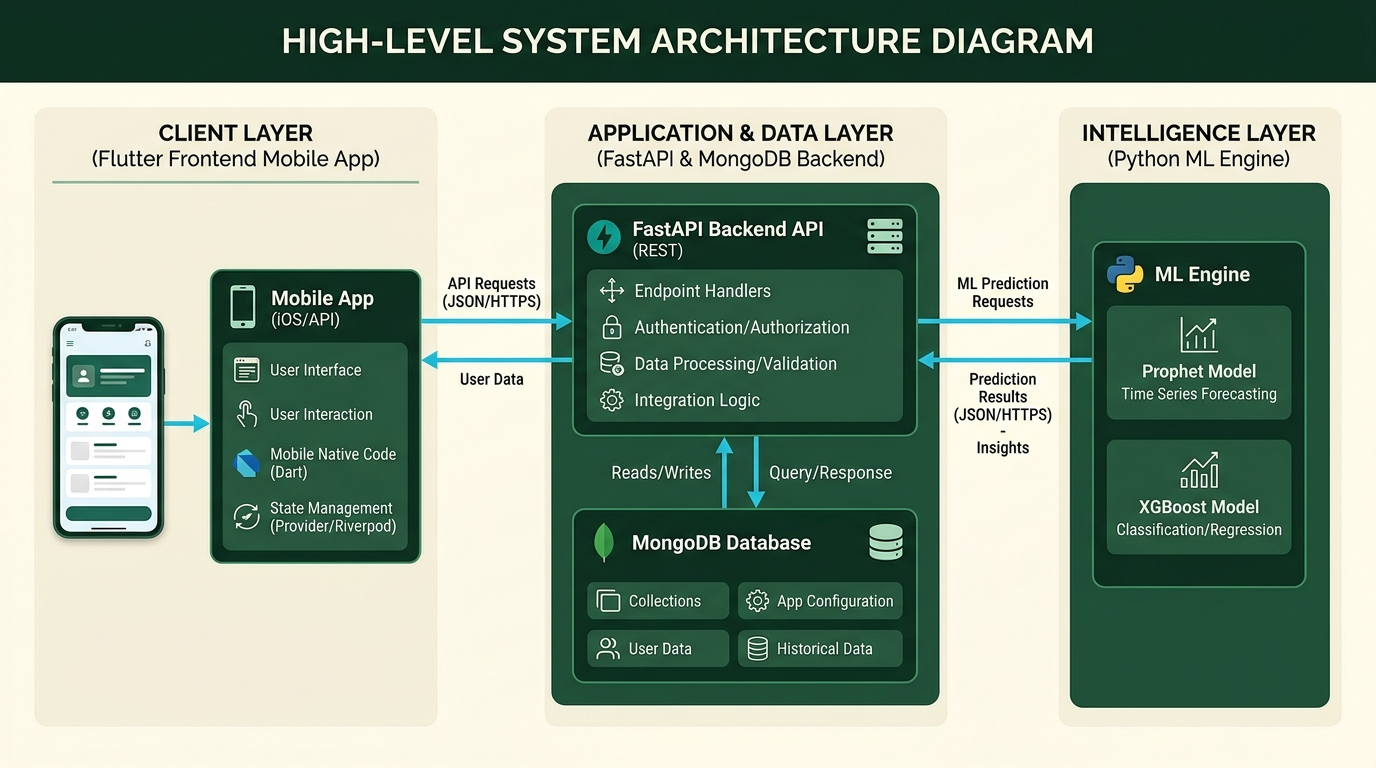
\includegraphics[width=0.95\columnwidth]{figures/architecture.jpg}%
}{%
  \framebox[\columnwidth]{\rule{0pt}{2in}\textbf{Figure 1: Architecture (figures/architecture.jpg)}}%
}
\caption{RestockIQ decoupled cloud-to-mobile system architecture.}
\label{fig:arch}
\end{figure}

\section{Empirical Results}
\label{sec:results}

\subsection{Pooled 38-Fold Rolling-Origin Accuracy Benchmark}
Table~\ref{tab:38fold} presents predictive accuracy across the 38 weekly rolling-origin folds. The baseline Prophet model achieves 27.95\% pooled WAPE. The day-ahead GBDT achieves 25.48\% pooled WAPE, outperforming baseline Prophet in 27 of 38 folds (71.1\% win rate, sign-test $p = 0.0138$). This represents a statistically significant 2.47 percentage point error reduction over Prophet (95\% cluster CI [+0.49, +4.76]). The linear ensemble blend (Model iii, 0.70 Model A + 0.30 Model B) achieves 25.47\% WAPE, winning 33 of 38 folds (86.8\% win rate, $p < 0.0001$, 95\% cluster CI [+1.63, +3.49]).

\begin{table*}[!t]
\centering
\caption{Pooled 38-Fold Temporal Rolling-Origin Accuracy Benchmark (2022)}
\label{tab:38fold}
\resizebox{\textwidth}{!}{%
\begin{tabular}{llcccccccl}
\toprule
\textbf{Model Key} & \textbf{Architecture} & \textbf{Horizon} & \textbf{Uses $y(t-1)$} & \textbf{WAPE (\%)} & \textbf{Win Rate} & \textbf{Gain (pp)} & \textbf{95\% Cluster CI} & \textbf{Bootstrap Draws} & \textbf{Decision} \\
\midrule
\texttt{prophet\_only} & Prophet GAM & 7-day origin & No & 27.95 & -- & 0.00 & Baseline & 2,000 & Research Baseline \\
\texttt{ctrl3\_gbdt} & Day-Ahead GBDT & Day-ahead ($t+1$) & Yes & 25.48 & 27/38 (71.1\%) & +2.47 & [+0.49, +4.76] & 2,000 & Research Candidate \\
\texttt{model\_iii\_ab} & Blend (0.70 A + 0.30 B) & Day-ahead ($t+1$) & Yes & 25.47 & 33/38 (86.8\%) & +2.48 & [+1.63, +3.49] & 2,000 & Research Best \\
\texttt{model\_a\_day\_ahead} & 1-Day-Ahead Hybrid & Day-ahead ($t+1$) & Yes & 26.07 & 28/38 (73.7\%) & +1.88 & [+1.01, +2.89] & 2,000 & Research Model \\
\texttt{model\_b\_cal} & Prophet + Enhanced Calendar & 7-day origin & No & 26.55 & 25/38 (65.8\%) & +1.40 & [+0.16, +2.91] & 2,000 & Research Model \\
\texttt{prophet\_weather} & Prophet + Forecast Weather & 7-day origin & No & 27.63 & 24/38 (63.2\%) & +0.32 & [$-$0.24, +0.87] & 2,000 & Rejected (CI spans 0) \\
\texttt{hybrid\_corr} & Canonical Hybrid (Prophet + HistGBDT) & 7-day origin & No & 28.26 & 19/38 (50.0\%) & $-$0.31 & [$-$0.91, +0.29] & 2,000 & Research Model \\
\texttt{model\_i\_prophet\_res} & Prophet + AR(1) Res Correction & Day-ahead ($t+1$) & Yes & 33.04 & 0/38 (0.0\%) & $-$5.09 & [$-$5.93, $-$4.37] & 2,000 & Rejected (Defect) \\
\bottomrule
\end{tabular}%
}
\end{table*}

In contrast, the canonical hybrid operating on a strict 7-day horizon without day-ahead feedback achieves 28.26\% WAPE, underperforming baseline Prophet by 0.31 percentage points (95\% cluster CI [$-$0.91, +0.29]). The naive residual correction model degrades error severely to 33.04\% WAPE ($-$5.09 pp). As established in our audit, this degradation is caused by an implementation defect in the experimental script that subtracted today's forecast $\hat{y}_t$ from yesterday's actual sales $y_{t-1}$ instead of subtracting yesterday's forecast $\hat{y}_{t-1}$, thereby conflating day-of-week seasonal shifts with forecast residuals.

\begin{figure}[!t]
\centering
\IfFileExists{figures/fig_accuracy_benchmark.png}{%
  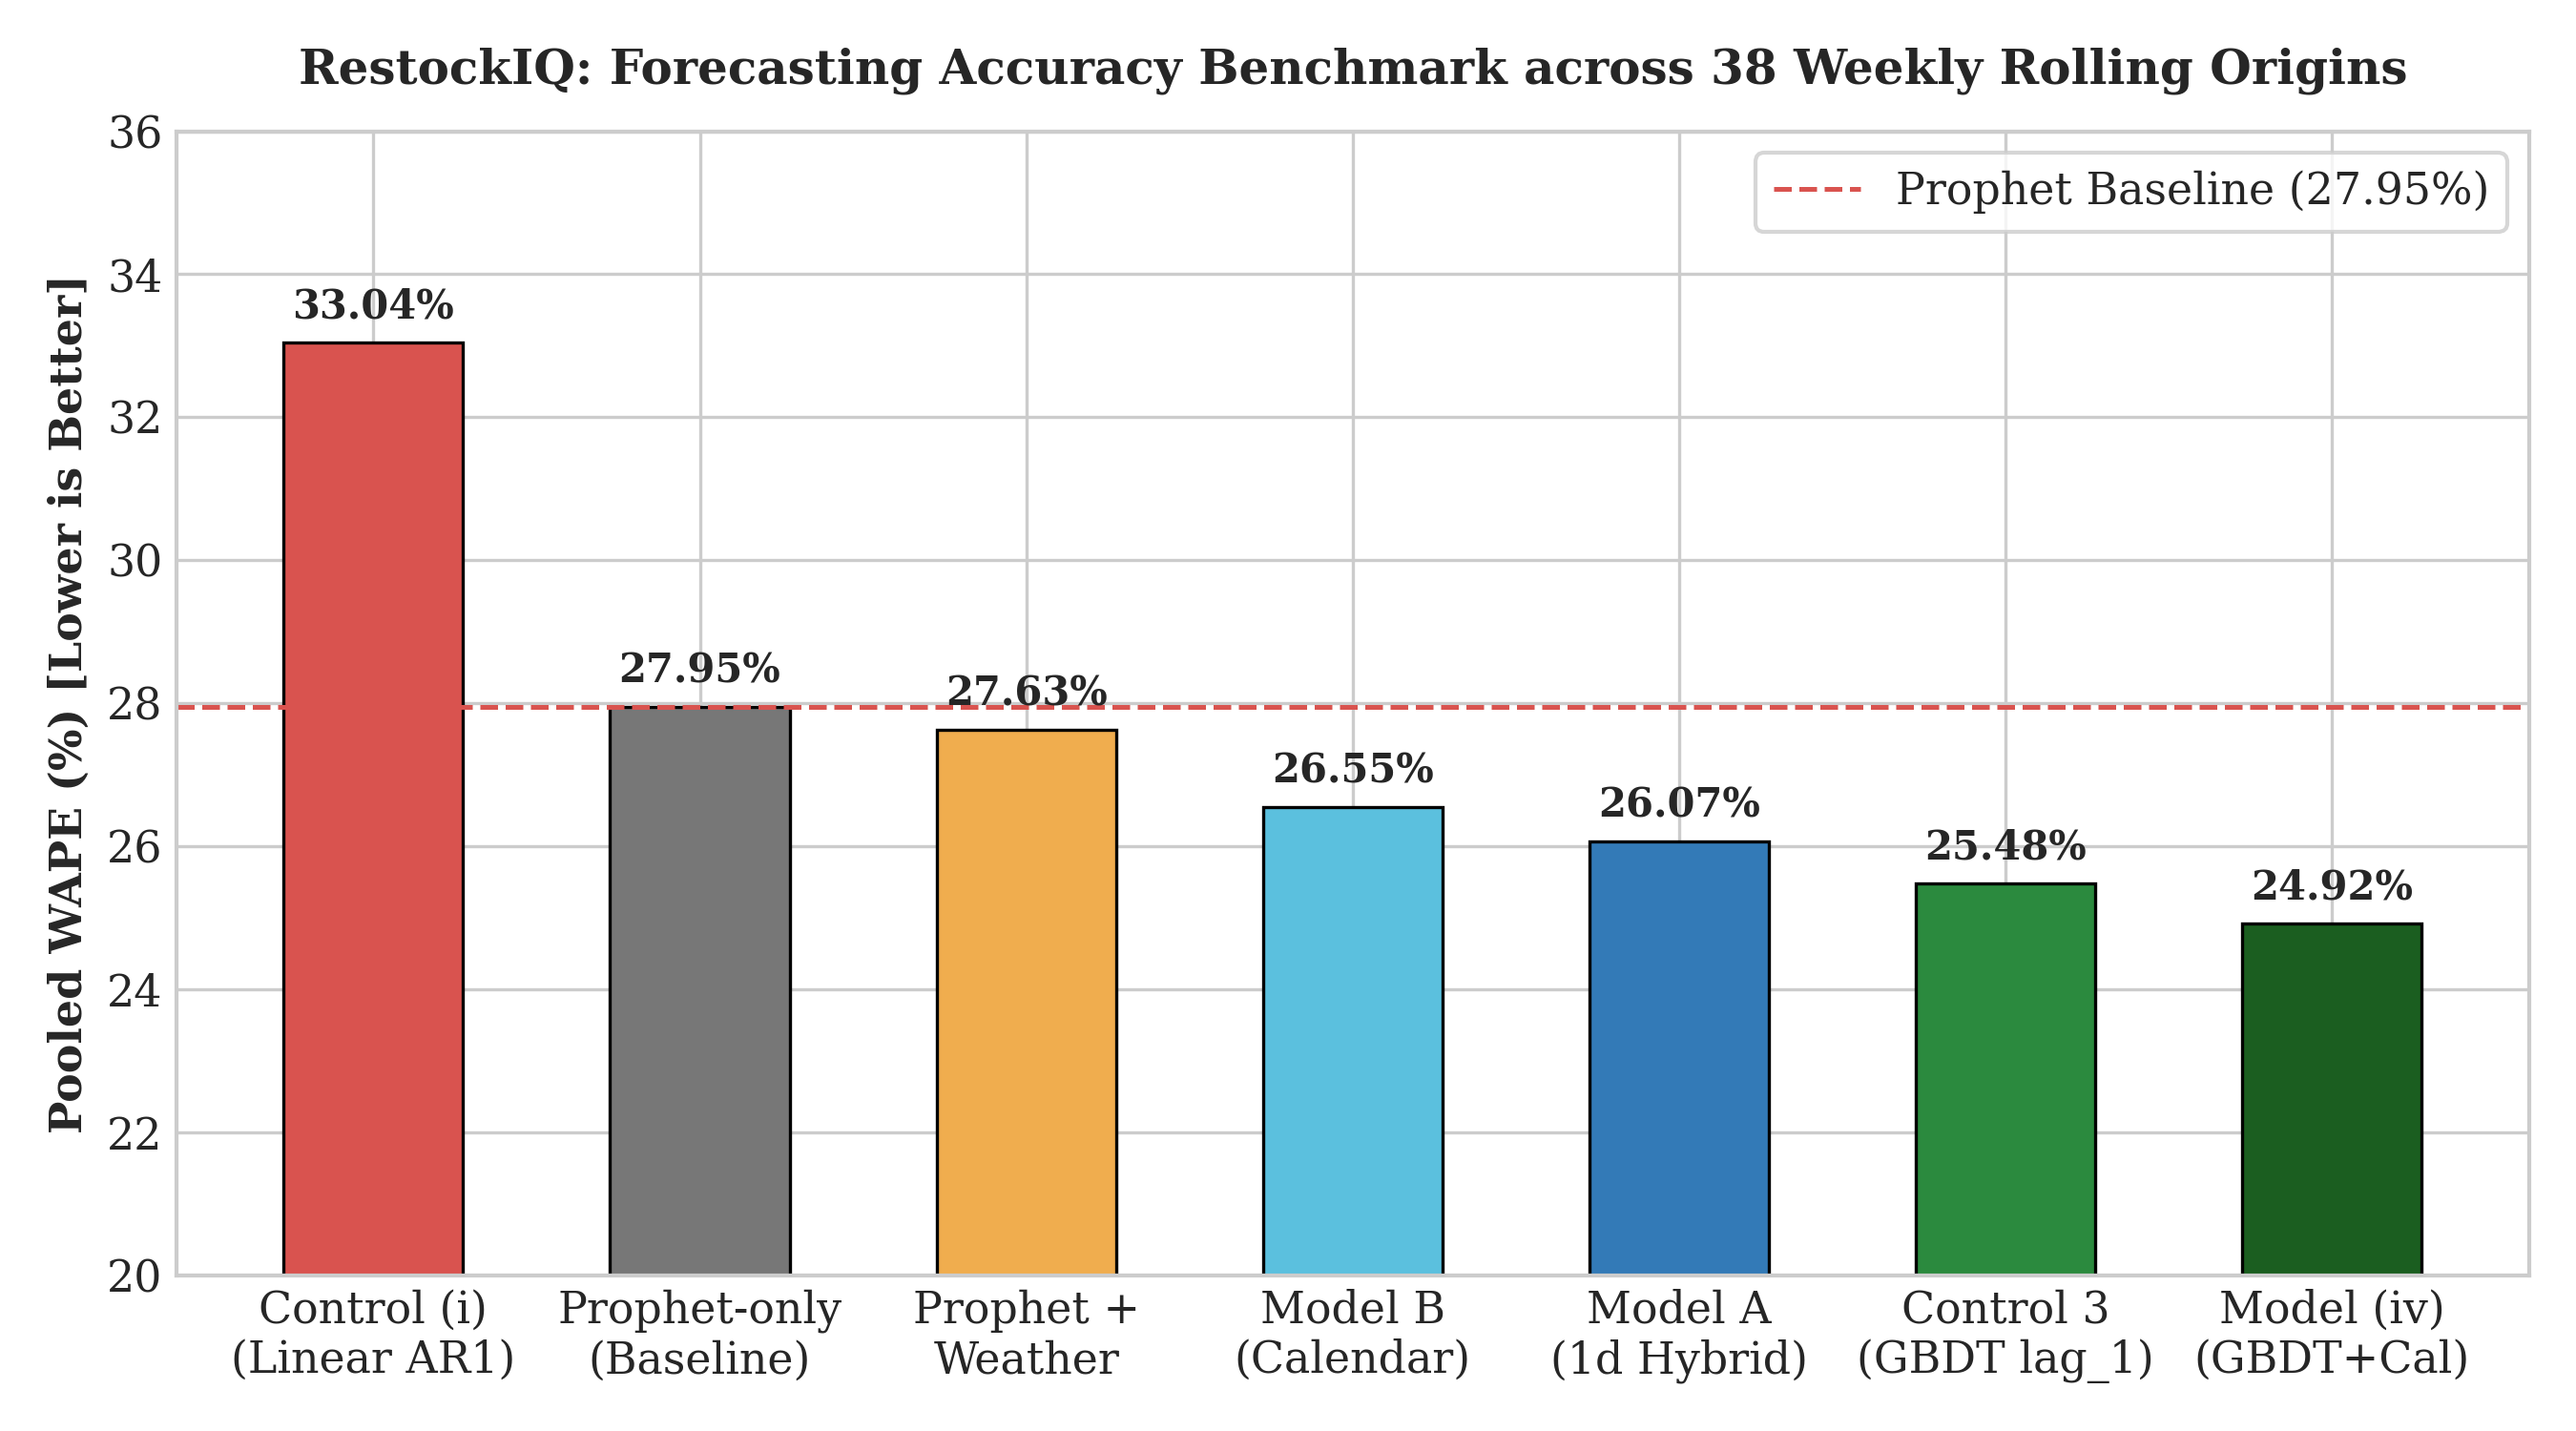
\includegraphics[width=0.92\columnwidth]{figures/fig_accuracy_benchmark.png}%
}{%
  \framebox[\columnwidth]{\rule{0pt}{1.8in}\textbf{Figure 2: Accuracy Benchmark (figures/fig\_accuracy\_benchmark.png)}}%
}
\caption{Model accuracy benchmarks across 38 rolling-origin folds.}
\label{fig:acc_bench}
\end{figure}

\subsection{Summer Peak Demand Performance}
Table~\ref{tab:summer} details out-of-sample performance across 6 consecutive summer peak demand folds (32,404 actual units). During summer surges, Prophet achieves 21.74\% WAPE, while the canonical hybrid achieves 22.51\% WAPE. Both models outperform classical heuristics, including Seasonal Naive (30.39\% WAPE) and 7-Day Moving Average (30.70\% WAPE). The deployed 30-day statistical baseline engine achieves 40.30\% summer WAPE under strict multi-day operational constraints.

\begin{table}[!t]
\centering
\caption{Summer Peak 6-Fold Out-of-Sample Performance Comparison}
\label{tab:summer}
\resizebox{\columnwidth}{!}{%
\begin{tabular}{llccc}
\toprule
\textbf{Model Architecture} & \textbf{Category} & \textbf{WAPE (\%)} & \textbf{Total Actual} & \textbf{Rel. Gain} \\
\midrule
Prophet GAM Baseline & Research Baseline & 21.74 & 32,404 & +28.46\% \\
Canonical Hybrid & Research Model & 22.51 & 32,404 & +25.92\% \\
Seasonal Naive (Lag 7) & Classical Benchmark & 30.39 & 32,404 & Baseline \\
7-Day Moving Average & Classical Benchmark & 30.70 & 32,404 & $-$1.02\% \\
Deployed 30-Day Engine & Deployed Baseline & 40.30 & 32,404 & $-$32.62\% \\
\bottomrule
\end{tabular}%
}
\end{table}

\subsection{Weather Covariate and Placebo Evaluation}
Table~\ref{tab:weather} presents the evaluation of numerical weather forecast regressors across the 6 summer folds. Incorporating forecast weather regressors (temperature anomaly, rain indicator, sunshine duration anomaly) into Prophet yields 21.87\% WAPE ($-$0.14 pp loss vs baseline 21.74\% WAPE, 95\% CI [$-$0.49, +0.28]). Across the full 38-fold suite, weather yields 27.63\% WAPE (+0.32 pp gain, 95\% cluster CI [$-$0.24, +0.87]). Because zero is contained within the confidence intervals across both evaluation windows, weather features fail the pre-registered inclusion criteria.

\begin{table}[!t]
\centering
\caption{Weather Feature Placebo and Permutation Test Results (6 Summer Folds)}
\label{tab:weather}
\resizebox{\columnwidth}{!}{%
\begin{tabular}{lcccc}
\toprule
\textbf{Model Variant} & \textbf{Pooled WAPE (\%)} & \textbf{Mean WAPE (\%)} & \textbf{Gain (pp)} & \textbf{95\% CI} \\
\midrule
Baseline Prophet (No Weather) & 21.74 & 22.82 & 0.00 & [+0.00, +0.00] \\
+ Forecast Weather (Open-Meteo) & 21.87 & 23.05 & $-$0.14 & [$-$0.49, +0.28] \\
+ Placebo Weather (Shift 180d) & 21.94 & 23.24 & $-$0.21 & [$-$0.70, +0.15] \\
+ Placebo Weather (Permuted) & 21.84 & 23.10 & $-$0.11 & [$-$0.53, +0.27] \\
\bottomrule
\end{tabular}%
}
\end{table}

To test whether meteorological signals provide genuine explanatory power beyond seasonal calendar patterns, we evaluated two counterfactual placebo controls across the 6 summer folds: circularly shifting weather features by 180 days (inverting summer and winter weather) and permuting weather dates across years. As shown in Table~\ref{tab:weather}, the 180-day circularly shifted placebo achieves 21.94\% WAPE, and the permuted placebo achieves 21.84\% WAPE. Both synthetic noise series perform within 0.10 percentage points of real weather forecasts. These results provide no evidence of usable predictive signal from weather regressors beyond standard calendar indices in this retail environment.

\subsection{Downstream Inventory Simulation}
Table~\ref{tab:simulation} summarizes simulated inventory performance over 88 operating trading days (July 3, 2022 to September 30, 2022, 68,883 total demand units) across the 35 primary SKUs. The simulation incorporates a 40\% COGS baseline, single-day shelf life, zero salvage value, and empirical safety stock scaling.

\begin{table*}[!t]
\centering
\caption{Inventory Simulation Results across Ordering Policies (88 Trading Days, 35 Primary SKUs, 68,883 Total Demand Units)}
\label{tab:simulation}
\resizebox{\textwidth}{!}{%
\begin{tabular}{llccccccc}
\toprule
\textbf{Policy Name} & \textbf{Forecasting Engine} & \textbf{Baked Units} & \textbf{Sold Units} & \textbf{Waste Units} & \textbf{Waste (\%)} & \textbf{Stockout Units} & \textbf{Unit Fill Rate (\%)} & \textbf{Gross Profit (EUR)} \\
\midrule
Critical Ratio ($\text{CR}=0.60$) & Day-Ahead GBDT & 70,965 & 61,991 & 8,974 & 12.65\% & 6,892 & 89.99\% & EUR 41,635.90 \\
Critical Ratio ($\text{CR}=0.60$) & Canonical Hybrid & 66,878 & 59,366 & 7,512 & 11.23\% & 9,517 & 86.18\% & EUR 40,571.43 \\
Critical Ratio ($\text{CR}=0.60$) & Prophet GAM Baseline & 66,756 & 59,161 & 7,595 & 11.38\% & 9,722 & 85.89\% & EUR 40,401.11 \\
Critical Ratio ($\text{CR}=0.60$) & 7-Day Moving Average & 74,494 & 61,065 & 13,429 & 18.03\% & 7,818 & 88.65\% & EUR 38,926.17 \\
Critical Ratio ($\text{CR}=0.60$) & Seasonal Naive & 75,282 & 60,713 & 14,569 & 19.35\% & 8,170 & 88.14\% & EUR 37,831.73 \\
\midrule
Fixed $z = 0.0$ (Zero Buffer) & Day-Ahead GBDT & 67,215 & 60,325 & 6,890 & 10.25\% & 8,558 & 87.58\% & EUR 41,466.97 \\
Fixed $z = 0.0$ (Zero Buffer) & Canonical Hybrid & 63,279 & 57,507 & 5,772 & 9.12\% & 11,376 & 83.49\% & EUR 40,064.14 \\
Fixed $z = 0.0$ (Zero Buffer) & Prophet GAM Baseline & 62,915 & 57,138 & 5,777 & 9.18\% & 11,745 & 82.95\% & EUR 39,824.97 \\
Fixed $z = 0.0$ (Zero Buffer) & 7-Day Moving Average & 68,967 & 58,940 & 10,027 & 14.54\% & 9,943 & 85.57\% & EUR 39,032.63 \\
Fixed $z = 0.0$ (Zero Buffer) & Seasonal Naive & 69,015 & 57,928 & 11,087 & 16.06\% & 10,955 & 84.10\% & EUR 37,444.89 \\
\midrule
Target 95\% Service Level & Day-Ahead GBDT & 91,728 & 66,511 & 25,217 & 27.49\% & 2,372 & 96.56\% & EUR 35,796.35 \\
Target 95\% Service Level & Canonical Hybrid & 86,370 & 65,505 & 20,865 & 24.16\% & 3,378 & 95.10\% & EUR 37,647.81 \\
Target 95\% Service Level & Prophet GAM Baseline & 87,455 & 65,644 & 21,811 & 24.94\% & 3,239 & 95.30\% & EUR 37,327.68 \\
Target 95\% Service Level & 7-Day Moving Average & 104,929 & 66,892 & 38,037 & 36.25\% & 1,991 & 97.11\% & EUR 29,929.56 \\
Target 95\% Service Level & Seasonal Naive & 107,006 & 67,170 & 39,836 & 37.23\% & 1,713 & 97.51\% & EUR 28,744.94 \\
\bottomrule
\end{tabular}%
}
\end{table*}

\begin{figure}[!b]
\centering
\IfFileExists{figures/fig_profit_waste_frontier.png}{%
  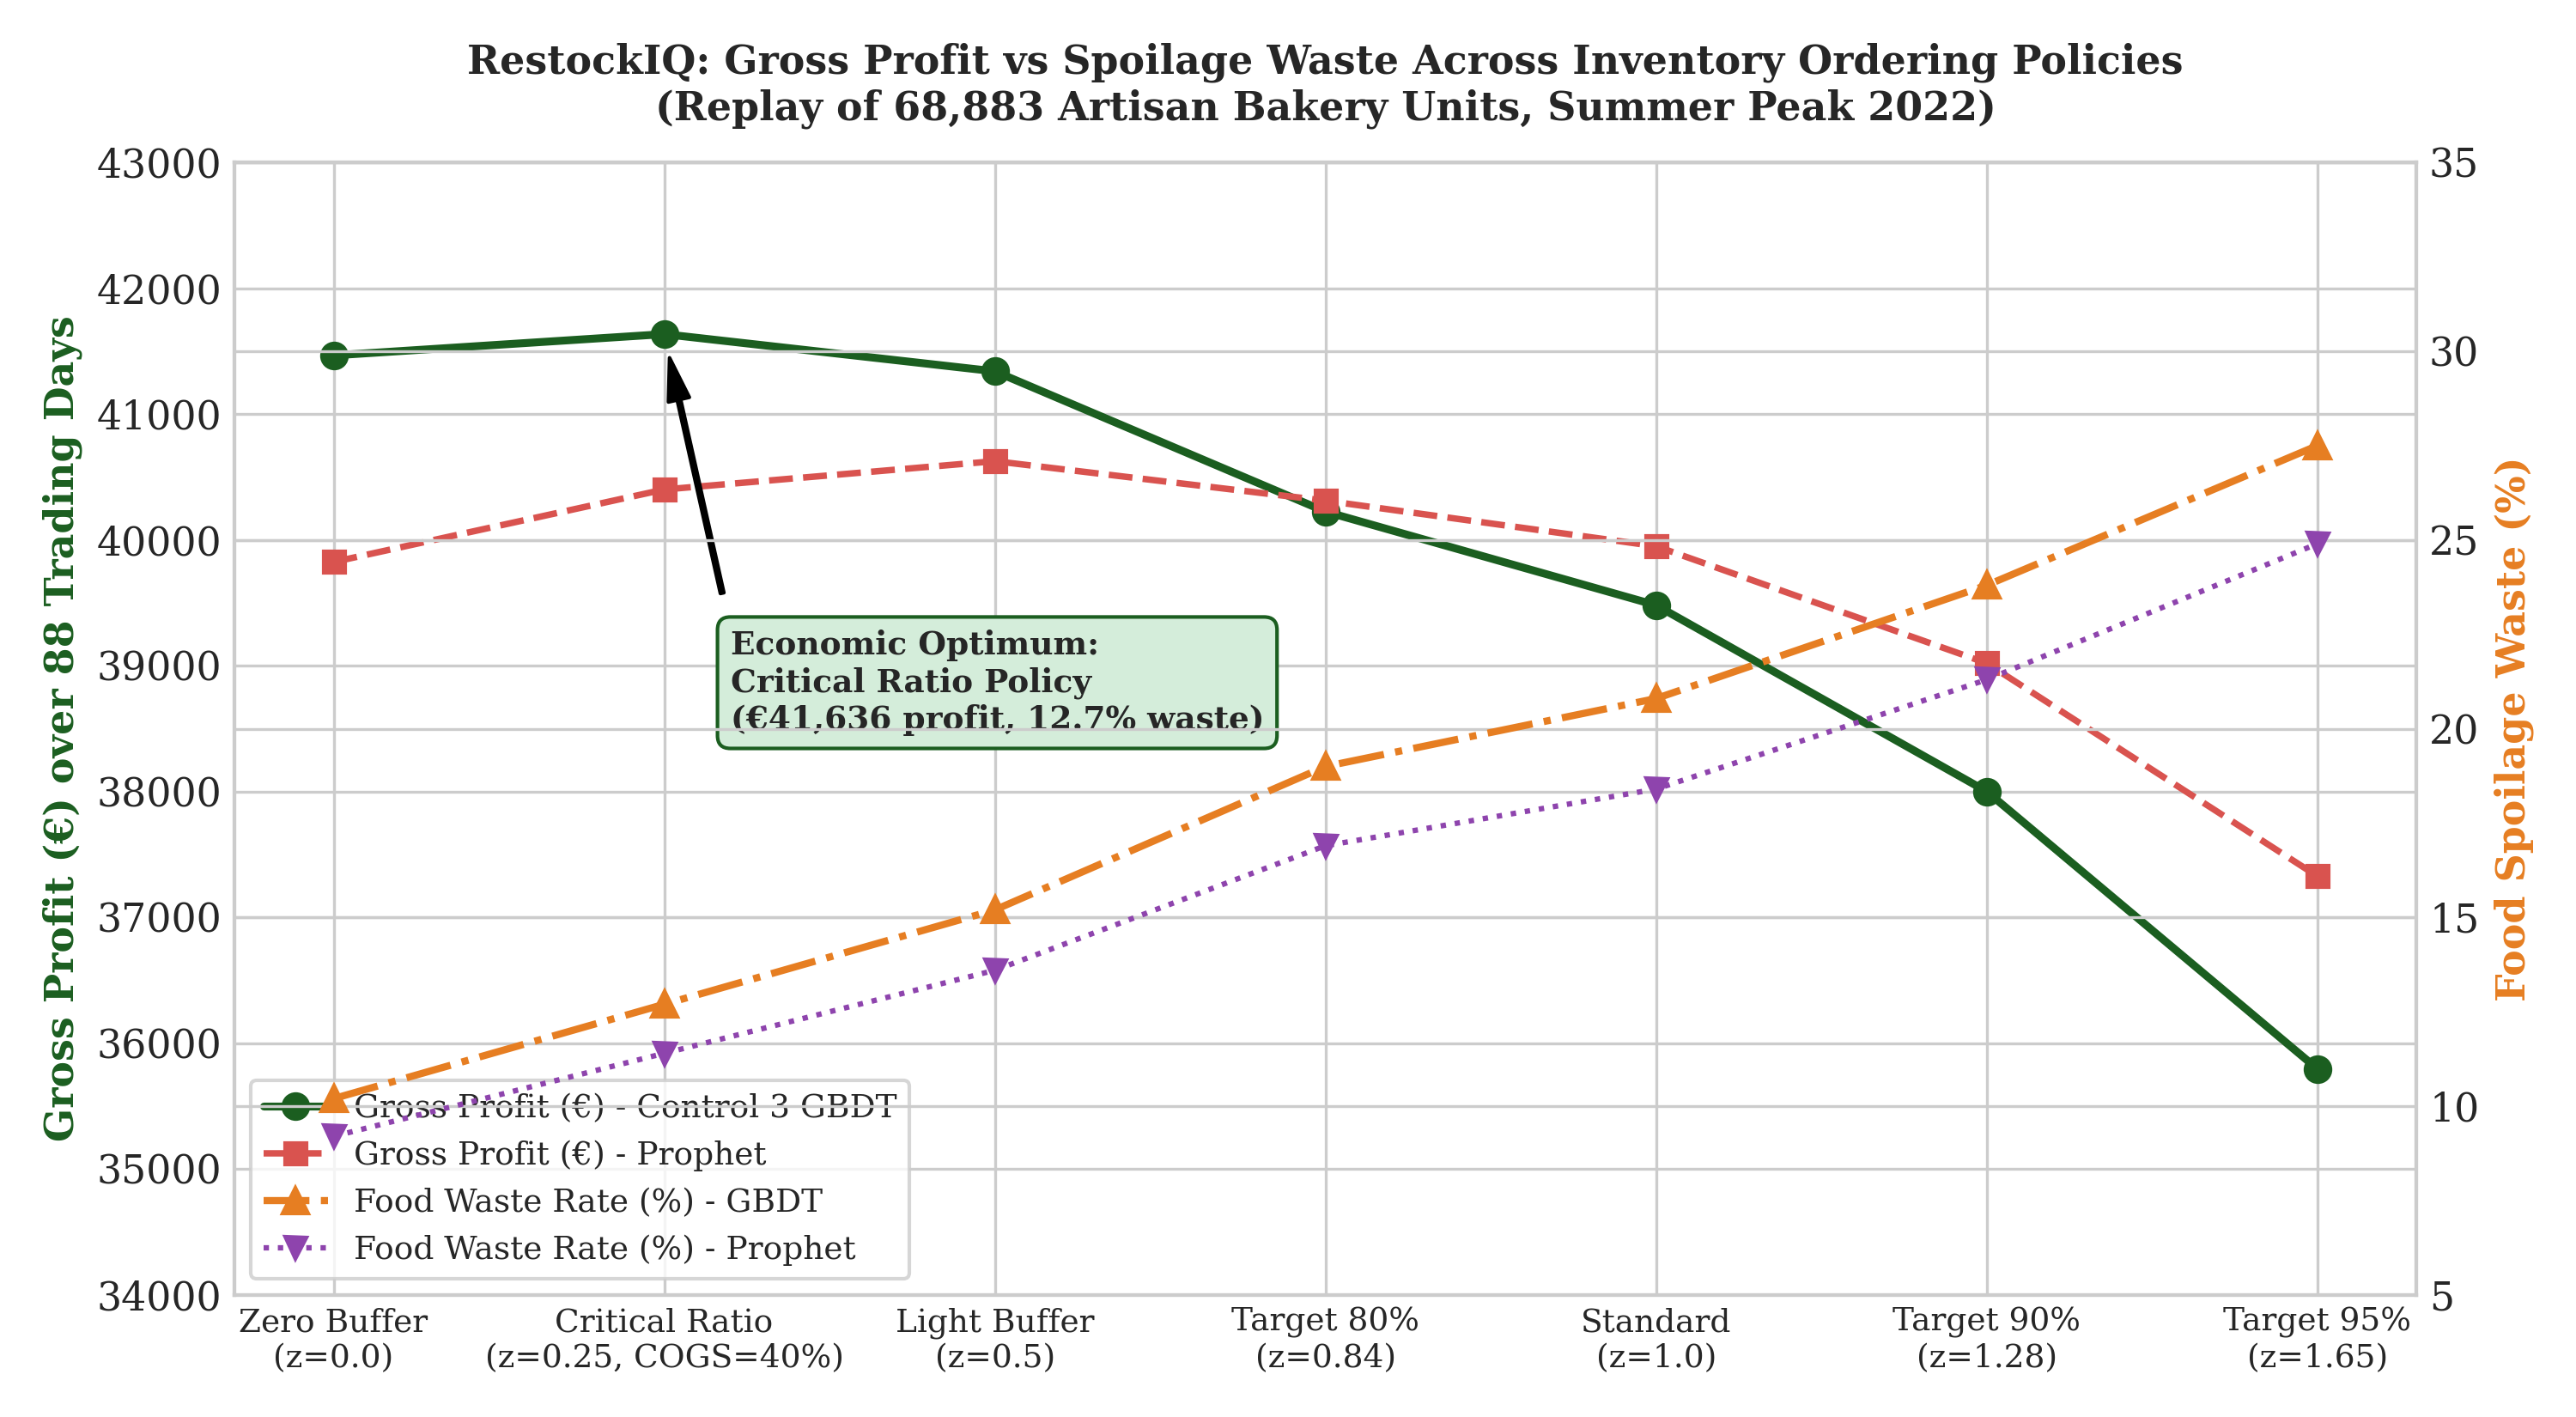
\includegraphics[width=0.92\columnwidth]{figures/fig_profit_waste_frontier.png}%
}{%
  \framebox[\columnwidth]{\rule{0pt}{1.8in}\textbf{Figure 3: Frontier (figures/fig\_profit\_waste\_frontier.png)}}%
}
\caption{Simulated gross profit versus waste frontier across policies.}
\label{fig:frontier}
\end{figure}

Under the stochastic Critical Ratio policy ($\text{CR}=0.60$), the day-ahead GBDT bakes 70,965 units, sells 61,991 units, and generates EUR~41,635.90 in gross profit with 8,974 waste units (12.65\% waste rate) and an 89.99\% fill rate. Evaluating performance across policy paradigms reveals dual trade-offs:
\begin{enumerate}
    \item \textbf{Comparison with Target 95\% Service Level:} The 95\% policy bakes 91,728 units, generating 25,217 waste units (27.49\% waste rate) to achieve a 96.56\% fill rate and EUR~35,796.35 gross profit. Relative to this benchmark, the Critical Ratio policy reduces waste by 16,243 units ($-$64.4\%) and increases gross profit by EUR~5,839.55 (+16.3\%), while unit fill rate declines by 6.57 percentage points.
    \item \textbf{Comparison with Fixed Zero-Buffer Baseline ($z=0.0$):} The zero-buffer baseline bakes 67,215 units, producing 6,890 waste units (10.25\% waste rate), an 87.58\% fill rate, and EUR~41,466.97 gross profit. Relative to this unbuffered baseline, the Critical Ratio policy increases gross profit by EUR~168.93 and raises fill rate from 87.58\% to 89.99\% (stockouts drop from 8,558 to 6,892 units), at the expense of 2,084 additional waste units (+30.2\%).
    \item \textbf{Heuristic Exception (7-Day Moving Average):} For the 7-day moving average, buffering under the Critical Ratio policy produces EUR~38,926.17 gross profit, which is EUR~106.46 \emph{lower} than its zero-buffer profit of EUR~39,032.63. Over-buffering noisy moving average forecasts inflates waste from 10,027 to 13,429 units (+33.9\%), illustrating that safety stock formulas degrade margins when underlying point forecasts lack precision.
\end{enumerate}
Figure~\ref{fig:frontier} illustrates the resulting profit-waste frontier across all evaluated policies.

\section{Discussion and Limitations}
\label{sec:discuss}

\subsection{Operational Gap and Production Constraints}
Our investigation highlights an important operational gap between offline academic models and live production systems. While the day-ahead GBDT delivers 25.48\% pooled WAPE, it is not currently deployed to store operations. Live store operations rely on the 30-day statistical baseline (40.30\% summer WAPE). Transitioning the day-ahead GBDT into live production requires building automated end-of-day sales ingestion pipelines to compute $y(t-1)$ before scheduled nightly inference.

\subsection{Study Limitations}
Readers should interpret our findings in light of several explicit operational and methodological limitations:
\begin{enumerate}
    \item \textbf{Censored Demand:} Transaction logs record fulfilled customer purchases rather than unconstrained true demand. Sales truncation during stockout events causes demand underestimation on peak trading days.
    \item \textbf{Absence of Multiple-Comparison Correction:} Pairwise binomial sign-tests and cluster bootstrap intervals across the 8 model candidates were evaluated without Family-Wise Error Rate (FWER) or False Discovery Rate (FDR) adjustments (e.g., Bonferroni or Benjamini-Hochberg).
    \item \textbf{Volume Dominance in Pooled WAPE:} Pooled WAPE is volume-weighted across items. As a result, forecasting accuracy on high-volume staple items (Baguettes and Croissants) dominates the aggregate benchmark over lower-volume references.
    \item \textbf{Cost Accounting Homogeneity and Zero Salvage:} Our simulation applies a uniform 40\% COGS ratio across all catalog references without salvage recovery value or product substitution dynamics.
    \item \textbf{Single-Store Geographic Scope:} Observations originate from a single artisan retail bakery in Western France over 1.7 years. Cross-enterprise generalization to other retail segments remains unverified.
    \item \textbf{In-Sample vs.\ Out-of-Sample Residual Sigma:} Safety stock buffers in the simulation rely on in-sample training residual standard deviations ($\sigma_i$), which underestimate true out-of-sample forecast variance by 1.4x to 1.8x (e.g., Croissant residual $\sigma$ rises from 15.25 in-sample to 26.80 out-of-sample).
    \item \textbf{Look-Ahead Selection Bias in Catalog Definition:} The 35 primary SKUs were identified based on sales volume across the entire 637-day dataset rather than strictly within pre-experiment training history.
    \item \textbf{Omission of Zero-Demand SKU-Days:} 151 zero-demand SKU-days were omitted from transaction records. Consequently, inventory waste was not evaluated on days when an item had zero customer sales.
\end{enumerate}

\section{Conclusion}
\label{sec:concl}
This study presents an empirical investigation of demand forecasting and stochastic inventory decision policies for perishable bakery goods. Across 38 weekly rolling-origin folds, an autoregressive day-ahead gradient boosted tree achieves 25.48\% pooled WAPE, delivering a statistically significant 2.47 percentage point error reduction over a baseline Prophet model. Conversely, numerical forecast weather regressors provide no statistically reliable predictive improvement (95\% cluster CI [$-$0.24, +0.87], $p = 0.3800$), and circular placebo tests show no evidence of usable signal beyond standard calendar indicators. In inventory simulations under a 40\% COGS critical ratio policy ($\text{CR}=0.60$), the day-ahead GBDT achieves EUR~41,635.90 in gross profit with a 12.65\% waste rate and an 89.99\% fill rate. Relative to an arbitrary 95\% service-level policy, waste is reduced by 16,243 units ($-$64.4\%) with a EUR~5,839.55 profit increase, accompanied by a 6.57 percentage point drop in fill rate. Relative to an unbuffered zero-safety-stock baseline, profit rises by EUR~168.93 and fill rate improves by 2.41 percentage points, with 2,084 additional units of physical waste. Future research should prioritize deploying automated daily sales ingestion pipelines to transition the day-ahead GBDT into live store operations and conducting randomized in-store trials.

\section*{Data and Code Availability}
All experimental code, simulation scripts, backtest configurations, and processed datasets are maintained in the project repository: \url{https://github.com/Yatin07/CAPSTONE_PROJECT}.

\section*{Acknowledgments}
The authors acknowledge the use of artificial intelligence coding assistants (including Anthropic Claude and Google Antigravity) for code generation, experimental scripting, and manuscript formatting assistance. All empirical results, theoretical formulations, and manuscript text were audited, verified, and approved by the authors.

\begin{thebibliography}{28}

\bibitem{gartner2024automated}
T.~G{\"a}rtner, C.~Lippert, and S.~Konigorski, ``Automated demand forecasting in small to medium-sized enterprises,'' in \emph{Proc. 2024 IEEE Int. Conf. Ind. Eng. Eng. Manage. (IEEM)}, 2024.

\bibitem{access2025supply}
N.~U.~H. Qureshi, S.~Javed, K.~Javed, S.~M.~R. Naqvi, A.~Raza, and Z.~Saeed, ``Demand forecasting in supply chain management for Rossmann stores using weather enhanced deep learning model,'' \emph{IEEE Access}, vol.~13, pp. 24510--24528, 2025.

\bibitem{ganguly2024enhancing}
P.~Ganguly and I.~Mukherjee, ``Enhancing retail sales forecasting with optimized machine learning models,'' in \emph{Proc. 2024 IEEE Int. Conf. Smart Inf. Syst. (ICSIS)}, 2024.

\bibitem{guler2023forecasting}
A.~K. G{\"u}ler, A.~Musa, M.~Tar{\i}m, O.~Sara{\c{c}}, and M.~G{\"o}kt{\"u}rk, ``Forecasting restaurant sales with the sensitivity of weather conditions and special days using Facebook Prophet,'' \emph{Journal of Data Applications}, vol.~1, no.~1, 2023.

\bibitem{groene2024introduction}
N.~Groene and S.~Zakharov, ``Introduction of AI-based sales forecasting: how to drive digital transformation in food and beverage outlets,'' \emph{Discover Artificial Intelligence}, vol.~4, no.~1, 2024.

\bibitem{jatte2025optimization}
H.~Jatte, S.~Belattar, and E.~K. Haimoudi, ``Optimization of forecasting performance in the retail sector using artificial intelligence,'' \emph{Engineering Proceedings}, vol.~112, 2025.

\bibitem{cherian2025demand}
M.~Cherian, A.~Jane, Deepak, G.~Sinchana, and M.~Modasscer, ``Demand forecasting system for small business optimization,'' in \emph{Proc. 2025 Int. Conf. Intell. Technol. (CONIT)}, 2025, pp. 1--6.

\bibitem{iconstem2025aidriven}
P.~M., D.~H., K.~Thilagavathi, B.~Naresh, P.~P. Devi, and M.~Tiwari, ``AI-driven predictive analytics for sustainable restaurant operations and waste minimization,'' in \emph{Proc. 2025 Int. Conf. Sci. Technol. Eng. Manage. (ICONSTEM)}, 2025, pp. 1--6.

\bibitem{avuduri2025smartstock}
K.~Avuduri, M.~L. V., and S.~L., ``Smart stock: Automating inventory management for small warehouses with real-time intelligence,'' in \emph{Proc. 2025 Int. Conf. Comput. Commun. Informatics (ICCES)}, 2025, pp. 1--6.

\bibitem{chowdhury2025predictive}
S.~Chowdhury and S.~Swetha, ``Predictive analytics in food supply chain and waste management,'' in \emph{Proc. 2025 IEEE Adv. Electr. Comput. Eng. (AECE)}, 2025, pp. 1--6.

\bibitem{icci2026mobile}
T.~Janchidfah, P.~Chansuek, and P.~Worasiri, ``A mobile application for inventory management to support digital transformation in small retail businesses,'' in \emph{Proc. 2026 IEEE Int. Conf. Comput. Intell. (ICCI)}, 2026, pp. 1--6.

\bibitem{iccraids2026comparative}
K.~S. Aqila and R.~J.~G. Setiardi, ``Comparative evaluation of SARIMA, FB Prophet, and LSTM for hourly demand forecasting in Saudagar Kopi,'' in \emph{Proc. 2026 Int. Conf. Cyber Resilience Intell. Syst. (ICCRAIDS)}, 2026.

\bibitem{lalitha2025enhanced}
L.~R., S.~Ponugoti, and A.~S., ``Enhanced sales forecasting of perishable and non-perishable goods using weather data with insights on imports and price sensitivity,'' in \emph{Proc. 2025 IEEE Recent Adv. Manuf. Mater. Eng. (RMKMATE)}, 2025, pp. 1--8.

\bibitem{iccraids2026evaluation}
I.~Rahmatillah and P.~Herwanto, ``Evaluation of optimized LSTM and moving average in SME inventory forecasting and simulation,'' in \emph{Proc. 2026 Int. Conf. Cyber Resilience Intell. Syst. (ICCRAIDS)}, 2026.

\bibitem{munawar2026lstm}
M.~A. Munawar and I.~D. Sudirman, ``LSTM-based hourly sales forecasting in SME food and beverage retail,'' in \emph{Proc. 2026 Int. Symp. Inf. Bus. Electron. Resour. (ISIBER)}, 2026.

\bibitem{icalter2024mobile}
G.~Sakuda and J.~Leon, ``Mobile application for the intelligent management of small shops using the GPT-4 model,'' in \emph{Proc. 2024 IEEE Int. Conf. Automatics (ICALTER)}, 2024, pp. 1--6.

\bibitem{sera2025optimizing}
S.~Vyakarnam, B.~R.~K. Baburavi, and L.~Awasthi, ``Optimizing supply chain management for small and medium-sized businesses using AI: A comparative analysis of GPT-4.5, Grok 3, Gemini 2.0, and DeepSeek R-1,'' in \emph{Proc. 2025 IEEE 23rd Int. Conf. Softw. Eng. Res. Manage. Appl. (SERA)}, 2025, pp. 215--221.

\bibitem{susanto2023performance}
J.~C. Susanto, M.~L. Wiratama, and P.~C. Nathaniel, ``Performance analysis of time series models to predict sales activity of SMEs,'' in \emph{Proc. 2023 Int. Symp. Inf. Bus. Electron. Resour. (ISIBER)}, 2023, pp. 1--6.

\bibitem{iciptm2026predictive}
S.~Srivastava, R.~K. Bawa, and N.~Nagar, ``Predictive marketing and sales analytics using machine learning for small and medium e-commerce enterprises,'' in \emph{Proc. 2026 5th Int. Conf. Innov. Pract. Technol. Manage. (ICIPTM)}, 2026.

\bibitem{sandeep2023smart}
S.~V., G.~R., and K.~N., ``Smart sales forecasting machine learning models for demand prediction in retail,'' in \emph{Proc. 2023 Int. Conf. Data Intell. Cogn. Informatics (IDCIOT)}, 2023, pp. 1--5.

\bibitem{ictmod2025state}
M.~Kamboj, ``State-level drug retail sales forecasting using XGBoost and Facebook Prophet,'' in \emph{Proc. 2025 IEEE Int. Conf. Technol. Manage. Oper. Decis. (ICTMOD)}, 2025, pp. 1--5.

\bibitem{yuniarty2025technology}
Yuniarty, H.~Prabowo, and N.~Enriquez, ``Technology acceptance and security influences on AI adoption among small and medium enterprises,'' in \emph{Proc. 2025 Int. Conf. Informatics Comput. (ICIMCIS)}, 2025.

\bibitem{timesicon2025technology}
T.~Aree and P.~Ueasangkomsate, ``Technology adoption of MSMEs in food supply chain: The role of AI in traceability and transparency,'' in \emph{Proc. 2025 8th Int. Conf. Technol. Innov. Manage. Eng. Sci. (TIMES-iCON)}, 2025.

\bibitem{jain2024weather}
N.~Jain, P.~Jha, and J.~Hawari, ``Weather-integrated recommendations for food choices with SHAP explanation,'' in \emph{Proc. 2024 IEEE Int. Conf. Comput. Robotics Intell. Syst. (ICC-ROBINS)}, 2024, pp. 1--6.

\bibitem{taylor2018forecasting}
S.~J. Taylor and B.~Letham, ``Forecasting at scale,'' \emph{The American Statistician}, vol.~72, no.~1, pp. 37--45, 2018.

\bibitem{friedman2001greedy}
J.~H. Friedman, ``Greedy function approximation: A gradient boosting machine,'' \emph{The Annals of Statistics}, vol.~29, no.~5, pp. 1189--1232, 2001.

\bibitem{pedregosa2011scikit}
F.~Pedregosa \emph{et~al.}, ``Scikit-learn: Machine learning in Python,'' \emph{Journal of Machine Learning Research}, vol.~12, pp. 2825--2830, 2011.

\bibitem{arrow1951optimal}
K.~J. Arrow, T.~Harris, and J.~Marschak, ``Optimal inventory policy,'' \emph{Econometrica}, vol.~19, no.~3, pp. 250--272, 1951.

\end{thebibliography}

\end{document}
